\chapter{Software Overview\label{sec:software}}

This chapter will serve as an overview of the functionality of the
\texttt{blcontrol} software. Figure~\ref{fig:ui} shows the full user interface
that appears when the application is started. Each panel in the window is
explained in its own section below.

%start software

\begin{figure}
\centering 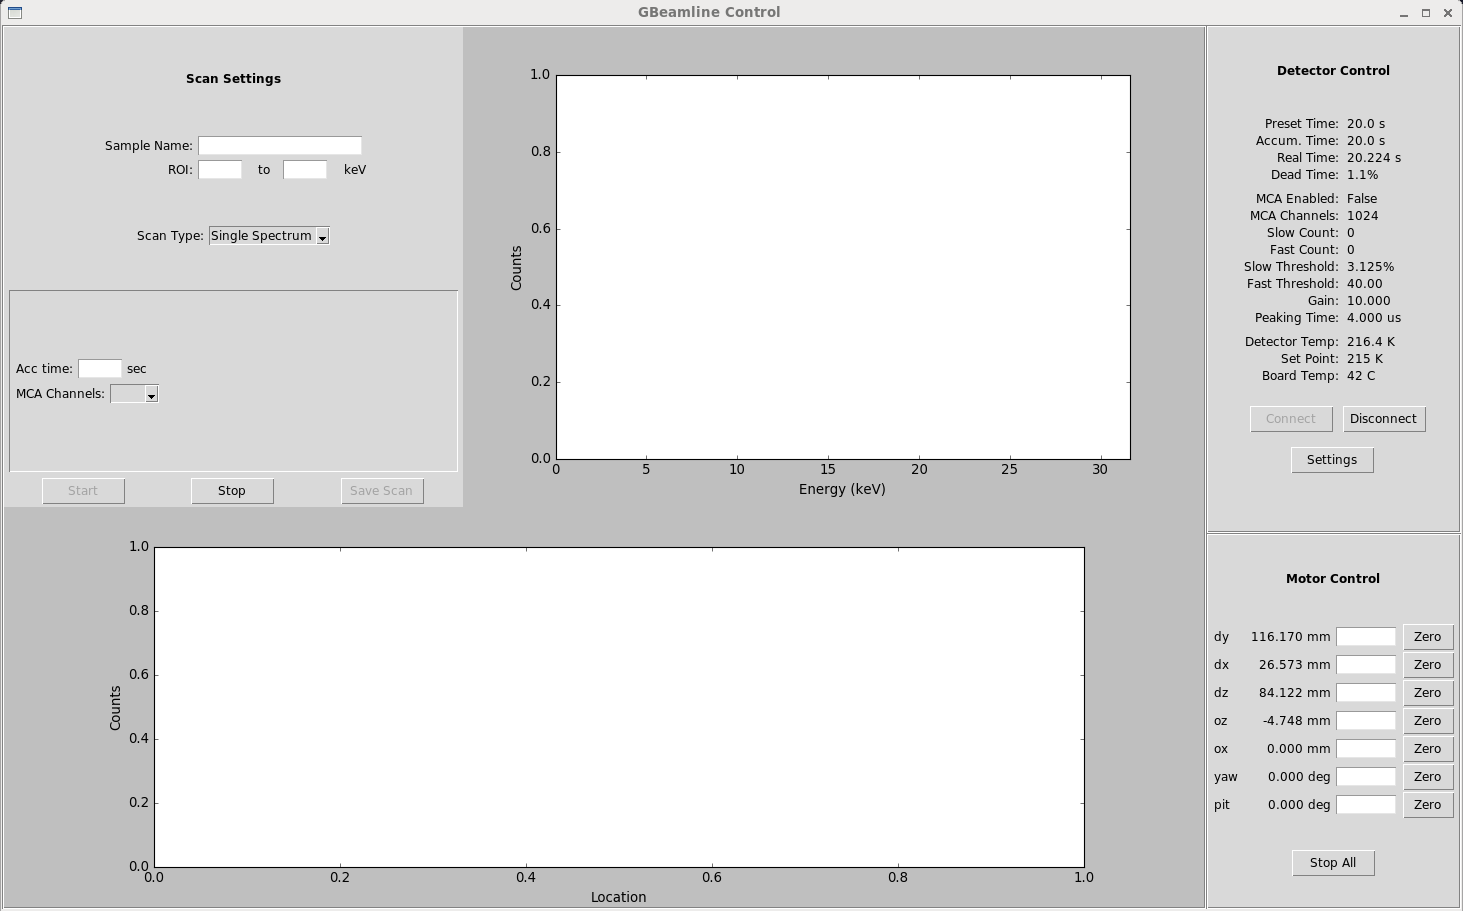
\includegraphics[width=\textwidth]{fullui.png}
\caption{\label{fig:ui} Screenshot of the full user interface on startup. The
  elements of the interface, clockwise from top left, are the scan settings, the
  single spectrum plot, the detector status readout, the motor control panel,
  and the scan plot.}
\end{figure}

\section{Scan Settings}

\begin{figure}
\centering 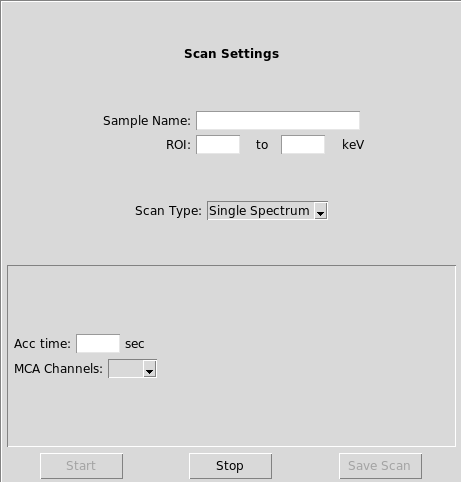
\includegraphics[width=0.45\textwidth]{scansettings.png}
\caption{\label{fig:scanset} The scan settings panel, with scan type set to
  ``Single Spectrum.''}
\end{figure}

The scan settings panel is shown in Fig.~\ref{fig:scanset}. The top half
contains fields for setting a sample name and ROI (region of interest) and a
drop-down menu for choosing a scan type.

The sample name field is only used to identify the sample in any saved
files. You can put whatever you like here or leave it blank.

The ROI setting allows you to choose a region of the spectrum between two energy
values to be analyzed in real-time along with the total spectrum. If this value
is set, the ROI will be highlighted in the spectrum plot and information about
the portion of the spectrum will be displayed on the plot. The counts in the ROI
will also be counted separately in any scans that are run.

The dropdown menu allows you to choose what type of scan to run, with the
choices being ``Single Spectrum,'' ``Linear Scan'' and ``Grid Scan.'' Each scan
type is covered in more detail below. When the scan type is changed, the lower
portion of the panel will change to display the settings available for that scan
type.  For each scan type, press the ``Start'' button on the bottom of the scan
settings panel to begin running the scan. The ``Stop'' button may be used to
terminate the scan prematurely. Once a scan is finished or has been stopped by
the user, the ``Save Scan'' button allows you to save the data from the most
recent scan in a plaintext format. The saved scan file will include all of the
detector status and settings data, and the current position of each connected
stage.

\subsection{Single Spectrum}

Fig.~\ref{fig:scanset} shows the layout of the scan settings panel when ``Single
Spectrum'' is selected. For a single spectrum, there are only two scan-specific
options: the accumulation time, in seconds, and the number of MCA channels to be
used. The accumulation time can be any value, and the number of channels is
selectable from a drop down menu. The detector allows the use of 256, 512, 1024,
2048, 4096, or 8192 channels.

\begin{figure}
\centering 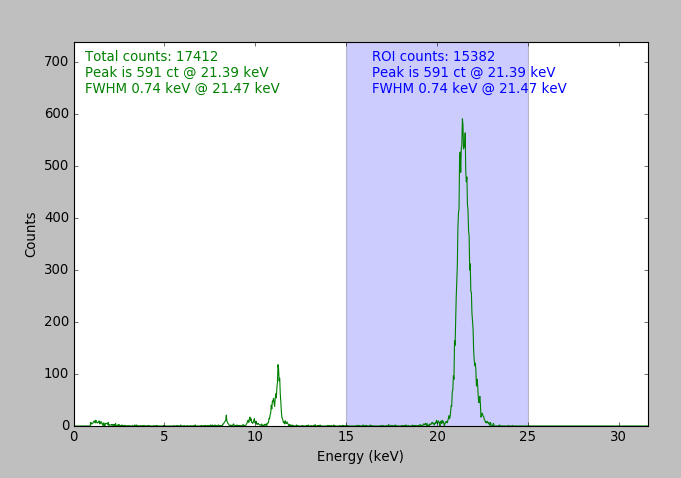
\includegraphics[width=0.7\textwidth]{specplot.png}
\caption{\label{fig:specplot} The spectrum plot display panel, during the
  collection of a single spectrum.}
\end{figure}

When the spectrum acquisition is started, after a few seconds the spectrum will
begin to display in the spectrum plot display panel, to the right of the scan
settings panel. This plot will update in real time (with the update frequency
depending on the number of channels) until the acquisition is complete.

An example image of the spectrum plot is shown in Fig.~\ref{fig:specplot}. In
the upper left corner, the green text displays some information about the
spectrum: the total number of counts, the number of counts and the location of
the peak channel, and the full width at half maximum (FWHM) and center of the
highest peak in the spectrum.  For this spectrum, the ROI was set to 15-25 keV,
and this region is highlighted in blue. The blue text in the upper right corner
gives the similar information about the portion of the spectrum that is
contained in the ROI. In this example, the highest peak in the ROI is the same
as the highest peak in the full spectrum.

\subsection{Linear Scan}

A linear scan consists of moving a single stage over a distance in specified
increments, and taking a spectrum at each position. This is useful during the
alignment process, when you want to position each stage at the location that
maximizes the count rate.

\begin{figure}
\centering 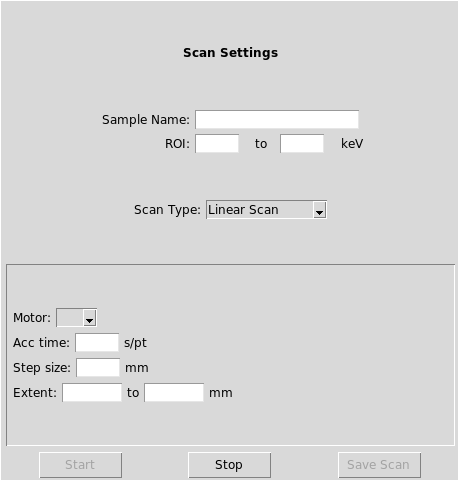
\includegraphics[width=0.45\textwidth]{linscan.png}
\caption{\label{fig:linscan} The scan settings panel when ``Linear Scan'' is
  selected.}
\end{figure}

Fig.~\ref{fig:linscan} shows the layout of the scan settings panel when ``Linear
Scan'' is selected. A dropdown menu allows you to choose a motor to scan from
the motors that are connected. The accumulation time field specifies the
duration of the spectrum that will be taken at each position. Step size is the
distance interval between each scan position. The default units are millimeters,
but will change to degrees if a rotary stage is selected from the motor dropdown
menu. Finally, the extent fields specify the beginning and ending points of the
scan. The extent is inclusive, meaning a spectrum will be taken at the beginning
of the interval, and, if the interval is exactly divisible by the step size, a
spectrum will be taken at the end of the interval as well. Together, the extent
and the step size define the number of points in a linear scan. The approximate
duration of the scan can be determined from the accumulation time at each point
and the number of points, but note that some extra time will be needed for data
transfer and stage motion.

%spec display
While the scan is running, the spectra collected at each point will be displayed
in the spectrum plot panel, similar to how it is displayed while collecting a
single spectrum. During a scan, however, the number of MCA channels is limited
to 256 to improve data transfer speed and decrease the size of the files
generated from the scans. When the scan is finished, the stage will remain in
the final location of the scan until moved by the user.

\begin{figure}
\centering 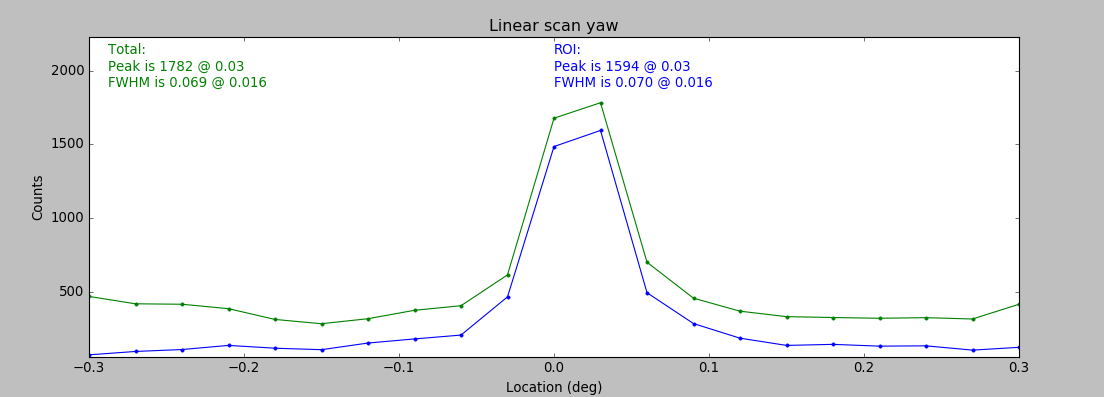
\includegraphics[width=\textwidth]{linplot.png}
\caption{\label{fig:linplot} The plot displayed in the scan plot display panel,
  after a linear scan is run.}
\end{figure}

%lin scan plot
A plot will also be generated in the scan plot panel, as shown in
Fig.~\ref{fig:linplot}. In real time during the scan, the plot will show the
total number of counts collected at each location in green, and the number of
counts in the ROI (if used) in blue. Information is also displayed about the
highest peak for both the total count data and the ROI data.

\subsection{Grid Scan}

A grid scan is a 2D scan of the detector in the $xy$ plane, which is useful for
centering the detector on the axis of the optic. Fig.~\ref{fig:gridscan}
displays the options for setting up a grid scan. The user specifies the
accumulation time as in a linear scan. The step size is the distance between
consecutive points in both the $x$ and $y$ directions. The grid size dropdown
menu allows the user to specify the number of points to be collected, from $3
\times 3$ to $11 \times 11$ points (odd numbers only).

\begin{figure}
\centering 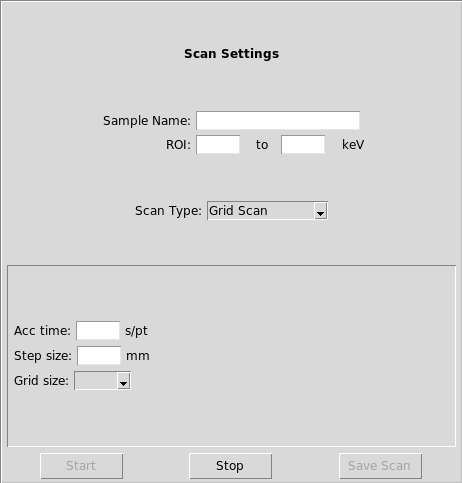
\includegraphics[width=0.45\textwidth]{gridscan.png}
\caption{\label{fig:gridscan} The scan settings panel when ``Grid Scan'' is
  selected.}
\end{figure}

Unlike the linear scan, which allows the user to specify the start and end
points of a scan, a grid scan is always centered around the position of the
detector at the time the scan is started. When the scan is initiated, the
detector will move to the first position, the lowest values of $x$ and $y$, and
proceed in a raster fashion until the scan is complete. First $x$ is scanned all
the way across in units of the step size, then $y$ is incremented by one step
and $x$ is scanned in the opposite direction, and so on until the entire area
has been scanned. As in the linear scan, the spectra appear in the spectrum plot
panel as they are acquired.

\begin{figure}
\centering 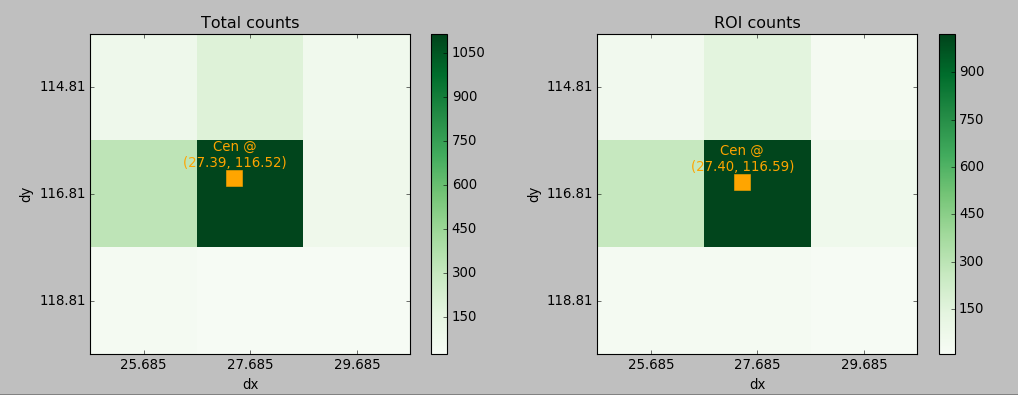
\includegraphics[width=\textwidth]{gridplot.png}
\caption{\label{fig:gridplot} The plot displayed in the scan plot display panel,
  after a grid scan is run.}
\end{figure}

The results of the scan are displayed in real time in the scan plot panel, shown
in Fig.~\ref{fig:gridplot}. Points are filled in as they are collected, and
points not yet collected appear in gray. The total counts are plotted on the
left, and the counts in the ROI, if used, are plotted on the right.  Both plots
display the calculated center of mass of the scans to aid the user in centering
the detector. When the scan is finished, the detector will remain at the final
point of the scan until moved by the user.

\section{Motor Control}

\begin{figure}
\centering 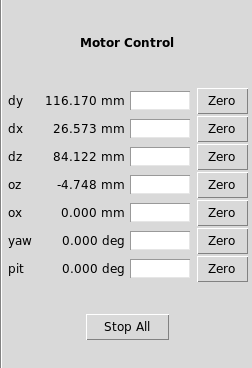
\includegraphics[width=0.35\textwidth]{motorctl.png}
\caption{\label{fig:motorctl} The motor control panel.}
\end{figure}

The user can move each stage independently using the motor control panel, shown
in Fig.~\ref{fig:motorctl}. For each connected stage, the current position is
shown, followed by a new position field and a ``Zero'' button. To move the stage
to a new position, enter the new position in the field and press Enter. The
current position will update in real time as the stage moves. You can also move
the stages using the hardware knobs. The zero button will set the current
position of the stage to zero. The ``Stop All'' button, located at the bottom of
the panel, can be used for an emergency stop of all stages.
% ^^ make sure to note that stage should be done moving before re-zeroing


%homing
If the power has been disconnected to one of the stages since the last use, it
must be homed before the next use, otherwise the encoder will not have a valid
position reference. If one or more of the motors is unhomed when the software is
started up, the user will be prevented from moving that motor. A warning message
will appear, the new position field for the affected stages will be grayed out,
and the ``Zero'' button will be replaced by a ``Home'' button. Pressing the
``Home'' button will instruct the stage controllers to perform the homing
routine automatically, but \textbf{you must make sure the area is clear for the
  motor to return all the way to the home position} before performing this
step. This includes ensuring that the stages will not run into any obstacles
while homing, and that the cables connecting the motors will not become tangled
or overstressed. Also, \textbf{the current position will be lost when the homing
  routine is performed}. For these reasons, it is often preferable to home the
motors manually, by using the knob on the controller to move them until the home
sensor is triggered. This allows you to move the motors slowly, make sure there
are no obstacles in the way, and mark the current position of the stages before
beginning the homing process.

%something about currents??

\section{Detector Control}

\begin{figure}
\centering 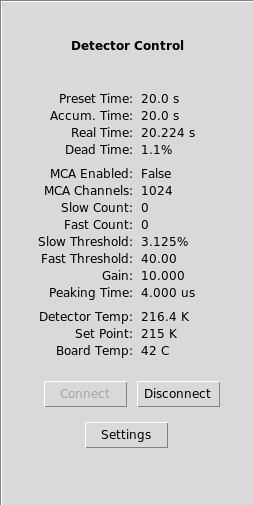
\includegraphics[width=0.3\textwidth]{detctl.png}
\caption{\label{fig:detctl} The detector status panel.}
\end{figure}

\subsection{Detector Status}

Figure~\ref{fig:detctl} shows the detector control panel. The top portion of the
panel displays constantly updated status information from the detector. The
preset time is the total duration for which the detector will accumulate the
current spectrum. ``Accum. Time'' is the amount of active accumulation time
elapsed so far in the current spectrum, and ``Real Time'' is the amount of real
(clock) time elapsed so far. The difference between the two is the dead time,
which depends on the count rate and the currently set peaking time in the
detector's pulse shaping electronics. More information about peaking time can be
found in the DP5 User Manual \cite[p.~8]{dp5_user_man}.

``MCA Enabled'' and ``MCA Channels'' give the current status of the detector's
multi-channel analyzer. ``Slow Count'' and ``Fast Count'' are the sum of all
counts in the slow and fast channels, respectively, and ``Slow Threshold'' and
``Fast Threshold'' are the currently set thresholds for the lower level
discriminator for the respective channels.  The DP5 User Manual discusses the
differences between the slow and fast channels \cite[p.~7-8]{dp5_user_man}. The
slow channel threshold is given in percent of the full energy range, and the
fast channel threshold is a number between 0 and 511.93, where 512 is the full
energy range (see \cite[p.~162]{dp5_prog_guide} for more information on the fast
channel threshold).  The total gain of the amplifier, which governs the energy
range of the MCA, is listed next. The status readout concludes with the total
gain of the preamplifier, the peaking time, the current detector temperature and
the set point of the detector cooler (in Kelvin), and the current temperature of
the electronics board (in degrees Celsius). The detector should be cooled to
below 225K. Lower temperatures are better for reduced noise.

Below the status readout are three buttons for interacting with the
detector. The primary purpose of the ``Connect'' and ``Disconnect'' buttons is
to re-establish communication if the detector stops responding or delivering
status updates. The detector communication port is opened and ready to be used
when the software is started.

\subsection{Modifying Detector Settings}

The ``Settings'' button in the detector control panel opens the ``Detector
Settings'' window, allowing the user to modify certain detector parameters. This
pop-up window is shown in Fig.~\ref{fig:detsettings}. On the left (``Basic'')
side, a number of commonly used settings are listed along with their current
values. To update one of the settings, modify the value in the text field and
then press the ``Apply'' button. If you have modified one or more of the values
in the text fields but you do not want to apply these changes, press the
``Reset'' button to reset all values to their previous settings.

The right side of the settings window, labeled ``Advanced,'' allows the user to
edit any of the ASCII configuration values for the DP5. All ASCII commands and
the allowed values for each are listed in the DP5 Programmer's Guide
\cite{dp5_prog_guide}. This function should not need to be used regularly, and
caution should be used when modifying the ASCII configuration.

To obtain the current value of an ASCII configuration parameter, enter the
4-character name of the parameter in the left text field and press the ``Get''
button. The parameter value will appear in the right text field. To change the
value of a parameter, enter the parameter name in the left text field and the
new value in the right field (after the ``='' sign). After setting a new value,
it is good practice to press ``Get'' again to verify that the desired value has
been set correctly.

\begin{figure}
\centering 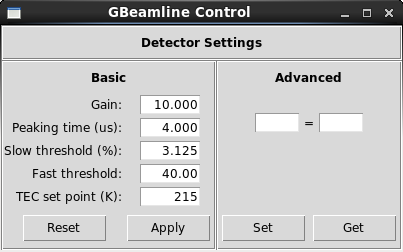
\includegraphics[width=0.5\textwidth]{detsettings.png}
\caption{\label{fig:detsettings} The detector settings popup window.}
\end{figure}

\section{Configuration Files}

Two configuration files are used by the \texttt{blcontrol} software. Both are
found in the \path{blcontrol/config} directory. The file \texttt{bldata.txt}
contains the zero positions for each stage in units of steps from the home
sensor. It should not need to be edited by the user, even when installing a new
stage. The software will automatically write to this file when the zero position
is changed by the user.

The second file is called \texttt{blconf.txt}. It is used by the software to
read various settings for the detector and motors, but it is not editable
directly in the software. When a stage or detector is modified or added to the
system, it will be necessary to edit \texttt{blconf.txt} to include the
specifications for the device, using a text editor. Note that if the
configuration file is modified, the software will need to be restarted for
changes to take effect. It is good practice to create a backup of your
configuration before making modifications so that you have a working version to
revert to if something breaks.

Sec.~\ref{sec:ex_conf} shows a recent version of this file for illustrative
purposes---the values listed there may not necessarily be valid for the current
iteration of the system. Each section heading is described in
Sec.~\ref{sec:conf_heads}. Note that \texttt{\#} indicates comments, \texttt{;}
indicates inline comments, section headings are indicated by \verb|[...]|, and
configuration values are listed as \verb|key=value|. Even if a device is not
currently connected to the beamline assembly, it can still have configuration
information listed in \texttt{blconf.txt} for future reference.

\subsection{Example \texttt{blconf.txt} \label{sec:ex_conf}}

\begin{verbatim}
# Beamline configuration file for motors and detectors 
# Last updated 10 April 2018

[Motor Names] 
36144=yaw 
36142=pit 
36153=dx
34795=dy
36592=dz
36900=ox
50852=oy
36610=oz
37203=rot3

[Motor Res] # Deg/step or mm/step, from zaber.com 
# Note: on motor spec sheets the resolution is given in mm or deg 
# per microstep at the default microstep resolution, which is 1/64.
yaw=0.015
pit=0.015
dy=0.003048
dx=0.003048
dz=0.03175
ox=0.006395
oy=0.006096
oz=0.0079375
rot3=0.01

[Max Current] 
# Amps 
yaw=0.95
pit=0.95
dy=0.5
dx=0.5
dz=0.55
ox=0.55
oy=0.95
oz=1.2
rot3=1.100

[Travel] 
# mm 
yaw= 
pit=
rot3=
dx=50.8
dy=152.4
dz=150
ox=150
oy=40
oz=254

[Stage Port] 
usbsn=AL00BUSL
serialport=/dev/ttyUSB0
timeout=5 ;seconds
baudrate=9600

[Detector Port]
timeout=10
serialport=/dev/ttyS0
baudrate=115200

##### Detector Calibration ##### 
# energy = (channel number)/((calib factor)*(hardware gain)*(num channels))
#  + offset 
# calib_factor units are 1/keV
# offset units are keV

[14845 Calib] 
#as of 10 April 2018 
calib_factor=0.00315691059703
offset=-0.0439739471587

[14711 Calib] 
#updated 12 sept 2016 with spectrum data from 9 sept 2016
calib_factor=0.000772012270785 
offset=-0.302908357512

[2607 Calib] 
#as of 20 April 2017 
calib_factor=0.000564960446259
offset=-0.104852853501

\end{verbatim}

\subsection{Configuration File Headings\label{sec:conf_heads}}

\subsubsection{Motor Names}

In this section each motor is listed by serial number and given a name which
will be used to identify it in the software and the rest of the configuration
file. A new \texttt{key=value} pair should be created for any new stage that is
introduced to the system, and the resolution, maximum current, and travel should
be defined in the following systems.

\subsubsection{Motor Res}

This section lists the resolution if each motor in real units, degrees per step
for rotary stages and mm per step for linear stages. These values are taken from
the specifications for each stage listed on \url{zaber.com}. As indicated in the
comments, the values in this configuration are in units/step, while the values
listed on the Zaber website are given in units/microstep.

\subsubsection{Max Current}

These are the maximum allowed values for the running and holding currents for
each motor from the specification sheet. The units are Amps.

\subsubsection{Travel}

This section lists the travel for each motor, in mm. Rotary stages have no limit
on travel (they are allowed to move past the home sensor), so this value is left
blank. This section also tells the software which units to use---a stage with no
travel defined is a rotary stage and therefore will use degrees instead of mm.

\subsubsection{Stage/Detector Port}

Settings for the communication port to the Zaber stages are listed under
\texttt{Stage Port}. The serial number of the USB-to-serial converter allows the
software to find the communication port automatically, or it must be specified
by the \texttt{serialport} variable. The timeout is user-definable and the units
are seconds. \texttt{baudrate} is the rate used when opening the port, and it
must match the baud rate that the stages are set to accept (this should not be
modified under normal circumstances).

The options for \texttt{Detector Port} are similar, except there is no USB
serial number because the detector communication is serial only.

\subsubsection{Detector Calibration}

This part of the configuration file consists of multiple sections, one for each
detector that is used in the beamline. The comments give the units of each
calibration variable and the instructions that the software uses to convert from
channel to energy using the calibration variables. Whenever a detector is
calibrated, the section corresponding to that detector's serial number must be
updated to reflect the new values of \verb|calib_factor| and \texttt{offset}. A
new section should be created for any new detector that is used in the system,
and it must have the heading \verb|[***** Calib]|, where \verb|*****| is the
serial number of the detector. Comment lines should always be given for each
detector to indicate when it was last calibrated. For more information on
calibrating the detectors, see Chapter~\ref{chap:calib}.
